\documentclass[sigconf]{acmart}

\usepackage{graphicx}
\usepackage{hyperref}
\usepackage{todonotes}

\usepackage{endfloat}
\renewcommand{\efloatseparator}{\mbox{}} % no new page between figures

\usepackage{booktabs} % For formal tables

\settopmatter{printacmref=false} % Removes citation information below abstract
\renewcommand\footnotetextcopyrightpermission[1]{} % removes footnote with conference information in first column
\pagestyle{plain} % removes running headers

\newcommand{\TODO}[1]{\todo[inline]{#1}}

\begin{document}

\title{Big Data Applications in Team Sports Predictive Analytics}
\author{Josh Lipe-Melton}

\orcid{1234-5678-9012}
\affiliation{%
  \institution{Indiana University}
  \streetaddress{4400 E Sheffield Dr}
  \city{Bloomington} 
  \state{Indiana} 
  \postcode{47408}
}
\email{jlipemel@umail.iu.edu}

\begin{abstract}
This paper showcases various models used in predictive analytics of sporting events
\end{abstract}

\keywords{sports, analytics, neural network, HID105, I523}

\maketitle

\section{Introduction}
The sports industry produces a lot of money, and because of this analysis of sporting events has become increasingly explored field. As technology improves, more and more data is generated regarding sporting events. Therefore, there have been numerous attempts to create functions that predict the outcomes of sporting events. Many efforts attempt to create neural networks to model these outcomes. Others use genetic pruning algorithms. Others break sporting events down into possessions and create a per possession model to predict the points scored by each competing party. Still more use a combination of all of these. By using various statistics, the results of a significant number of games can be predicted.

\section{Expected Goals Model}
Arguably the most common method of predicting the results of soccer games is to create a prediction of the number of goals scored by each team . The result of subtracting these two numbers gives not only a prediction of which team will win, but an inherent level of confidence proportional to the difference of each predicted number of goals \cite{ExpectedGoals}. This model creates an ''expected goals value'' by predicting the number of shots and assigning each of these shots a value. These values are based on attributes such as angle from the goal, distance to the goal, body part used to take the shot, what type of approach was used to obtain the shot (dribble, short pass, long pass, etc.), and even the relevant FIFA video game ratings of the player taking the shot. Each value represents the predicted likelihood of scoring, with 0 being an impossible shot and 1 being a sure goal. By summing these values and incorporating the FIFA rating of the opposing goalkeeper, an expected goals value for a team is obtained. The full list of features in this model is described in figure 1. This model is able to predict the number of goals scored by each team about 20 percent of the time. The correct result of the match was found about 56 percent of the time\cite{ExpectedGoals}. 

\begin{figure}[h!]
\centering
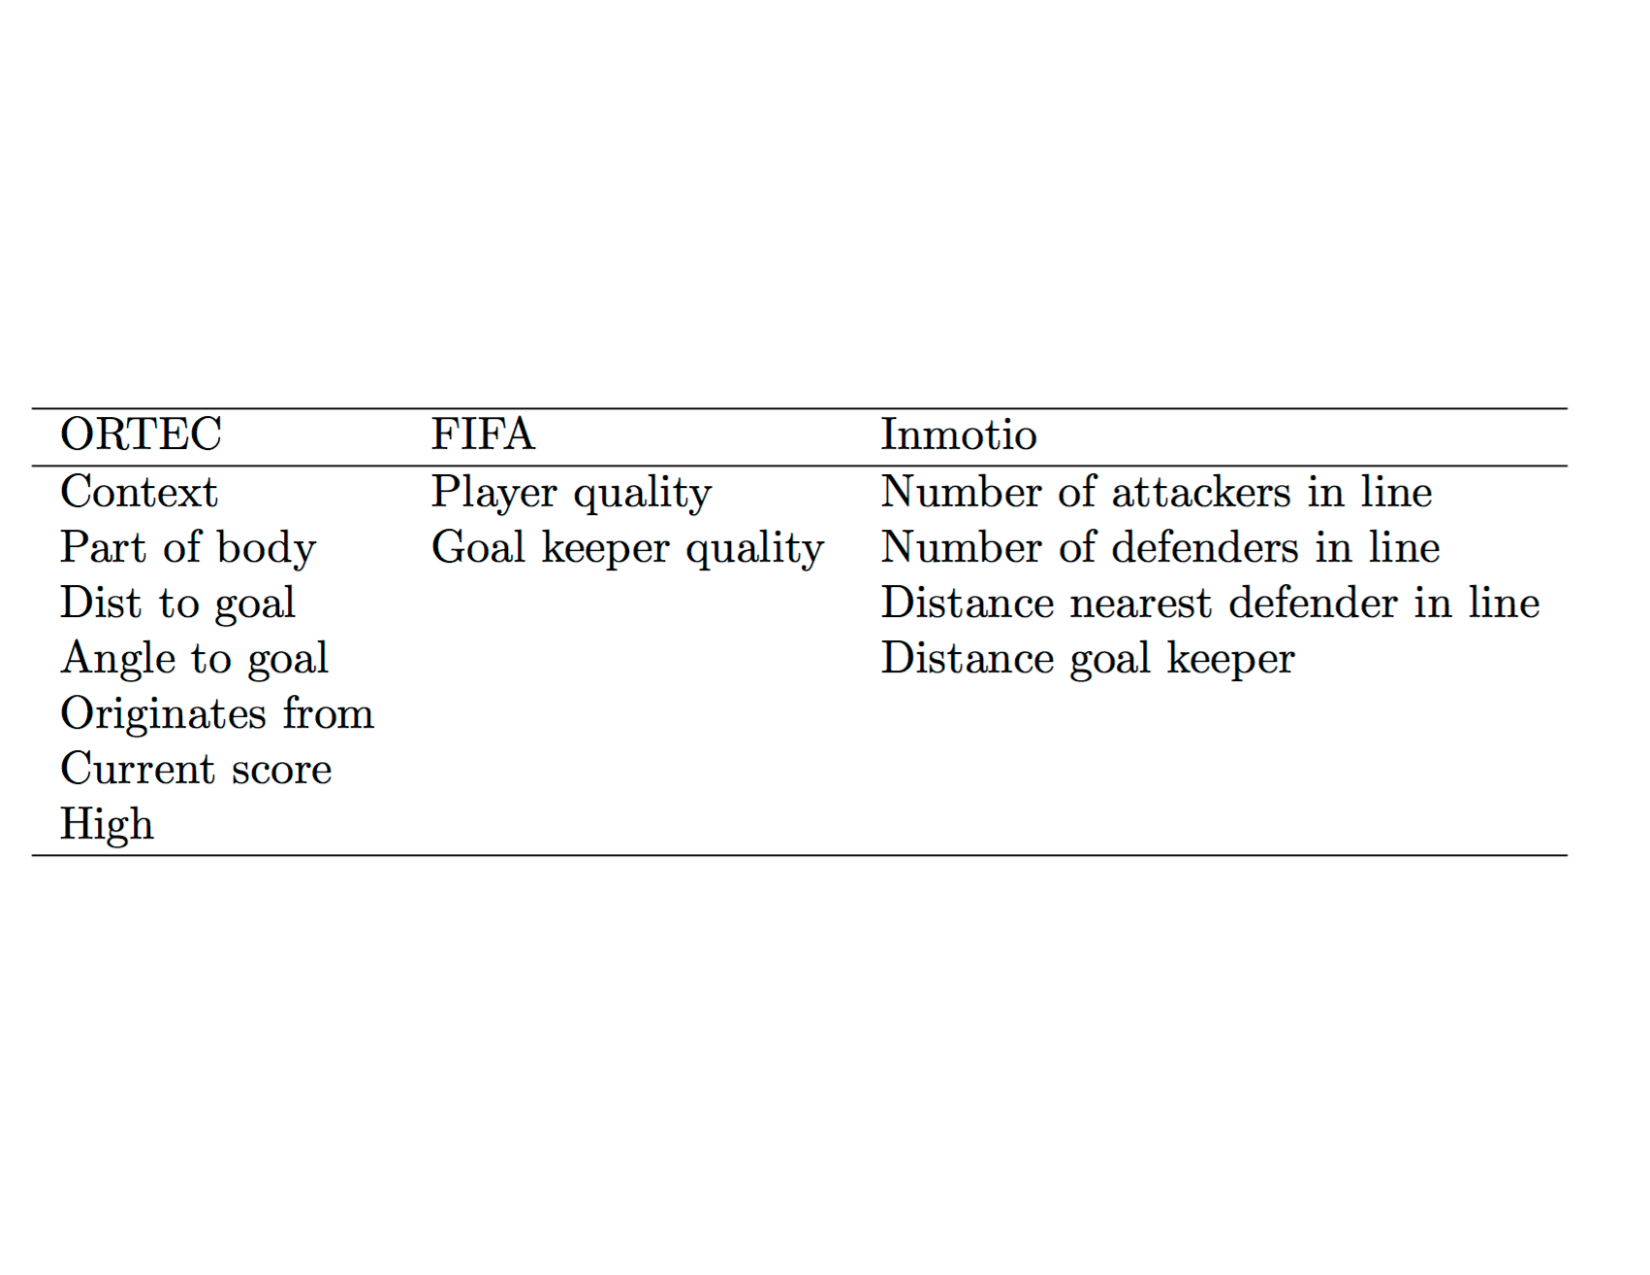
\includegraphics[scale=.2]{features.pdf}
\caption{Features of Expected Goals Model \cite{ExpectedGoals}}
\label{fig: Features of Expected Goals Model}
\end{figure}

\subsection{Bivariate Expected Goals Model}
A flaw with the previous example of an expected goals model is that it accounted only for the attack team's ability in its goal predictions. Apart from the ability of the goalie, there is no accounting for the defensive ability of an opponent in prediction of expected goals. In a different model, defensive ability and attacking ability are both incorporated. The authors of this method created their model based on the idea that the goals scored two competing soccer teams are negatively correlated with one another. By using a bivariate Poisson model for soccer data, the authors created predictions for the number of goals scored by each team in a given match, and therefore the results of each game\cite{BivariateExpected}. The covariates used in the bivariate Poisson regression model include: GDP per capita, population, home advantage, bookmaker's odds, market value, number of Champion's League players, number of club teammates, and the age of the coach. By running 1,000,000 simulations on the European Championships in 2016, predictions for each match were created, along with odds for each team to reach each round of the tournament. The odds of the model outperformed bookmakers' odds 42.22 percent to 39.23 percent in predictive accuracy\cite{BivariateExpected}. The authors used their model in placing equal bets on every bet in the tournament with the service that provided the most favorable odds to the outcome predicted by their model. In doing so, they obtained a return of 30.28 percent after the tournament.The authors concluded that the scores of two soccer teams are indeed negatively correlated and that this is a sound notion to base a predictive model on\cite{BivariateExpected}.

\section{Neural Network Method Using Past Match Results}
Another method of prediction solely uses past results to predict future results. In this method, a predictive model is based on the intuitive proposition that if team 1 has won their previous few games, team 2 has lost their previous few games, and team 1 has beaten team 2 the last two times they have played, team 1 will beat team 2\cite{FuzzyModel}. The model proposed in this article assigns a value in the range [-5, 5] to the last five games played by each team as well as the last two games played between the two teams. The higher the number, the bigger the win. The lower the number, the bigger the loss. The predicted result of a game is a function of these numbers. Through a combination of a fuzzy logic table and a neural network algorithm, a result is predicted. First, the authors created a table with every possible value of x1-x12. Each of these combinations was then associated with a predicted result and a weight in the interval [0, 1] that indicated the confidence in the predicted result. These initial confidence intervals were then tuned  The predicted result is drawn from the range [Big loss (BL), Small loss (SL), Draw (D), Small win (SW), Big win (BW)]\cite{FuzzyModel}. Using a sample size of 1056 matches, the source'' assigned weights to the nodes in the neural network as in Figure 2. The trained model was applied to 350 results from other seasons and was correct when predicting a big loss 91.4 percent of the time, a small loss 83.3 percent of the time, a draw 87 percent of the time, a small win 84 percent of the time, and a big win 94.6 percent of the time\cite{FuzzyModel}. This model greatly outperforms the previous model examined. However, the authors do cite flaws that come from not considering factors such as injured or suspended players, refereeing, or weather conditions \cite{FuzzyModel}.

Furthermore, this method's already impressive predictive accuracy could also be improved by taking into account strength of schedule, as a team that has narrowly won its last five games against very weak opponents would be favored against a team that has narrowly lost against very strong opponents. The machine learning techniques implemented in this study could have been improved by incorporating opponents' results into the model, giving more weight to wins against good teams.

\begin{figure}[h!]
\centering
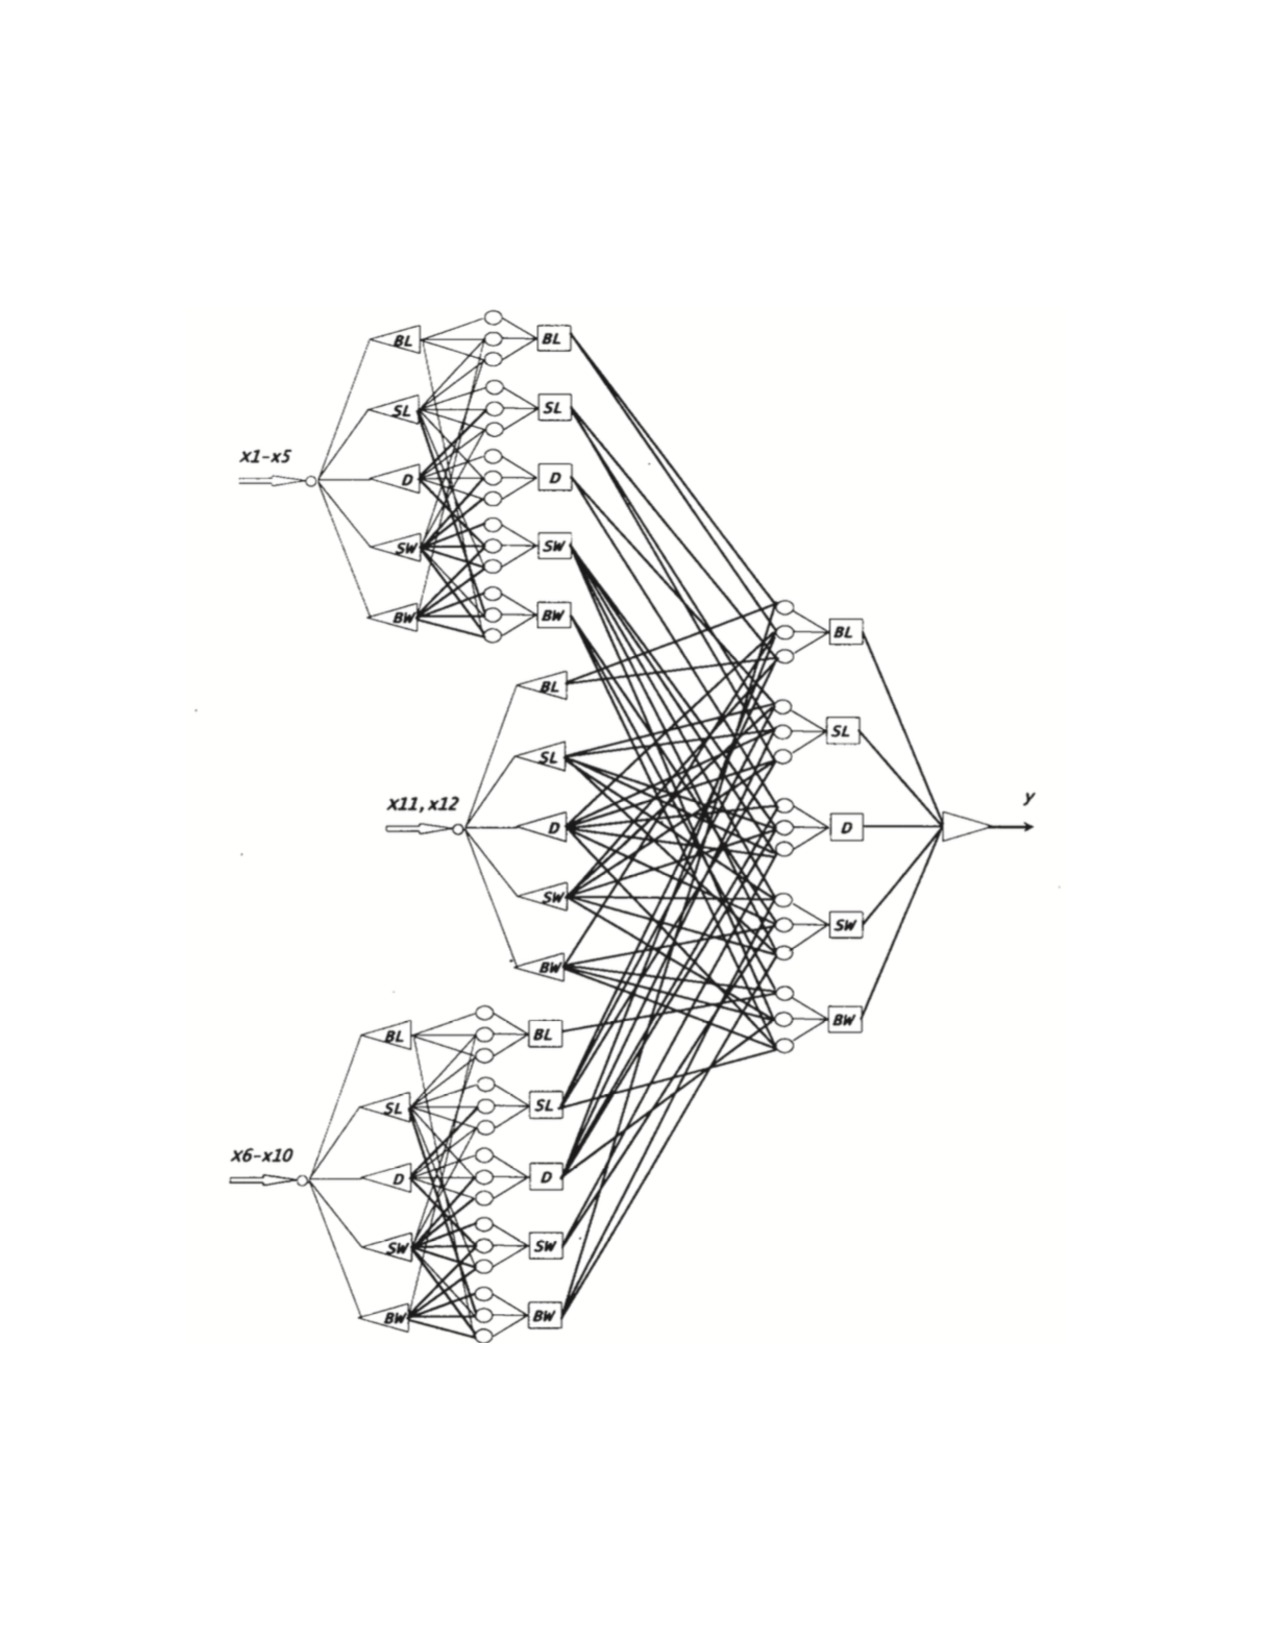
\includegraphics[scale=.5]{neuralnetworkdiagram.pdf}
\caption{Depiction of the neural network algorithm. x1-x5 and x6-x10 represent the results from each team's last five games, while x11 and x12 represent the results from the previous two games between the teams \cite{FuzzyModel}}
\label{fig:Nerual network depiction}
\end{figure}

\section{NCAA Analysis}
In college basketball, the committee that decides who gets into the NCAA tournament makes use of a ranking system called Ratings Percentage Index, or RPI. RPI weights .25 of a team's ranking on their win percentage, .5 on their opponents' win percentage, and .25 on their opponents' opponents' win percentage. \cite{RPI} This system is designed to encourage teams to schedule difficult opponents, as a large portion of the rankings is based on strength of schedule.
This formula has significant influence on where teams are ranked. Unfortunately, ''the RPI lacks theoretical justification from a statistical standpoint.'' \cite{RPI} In general, it is believed that the model places too much emphasis on strength of schedule and not enough on performance. Attempts to utilize an improved version of this model have made an impact on seeding in college soccer and baseball as well. In these sports, wins are weighted to give more ranking points to an away win than a home win.\cite{RPI} These types of alterations, however, do not address the fact that 75 percent of this ranking comes from a team's strength of schedule. This type of bias favors teams that are in strong conferences, even if they have poor records in their conference. 

\subsection{Per Possession Analysis}
A proposed alternative to RPI is to use a ''per possession model,'' or a model that predicts outcomes using statistics that are used in the context of efficiency with possessions. For example, offensive efficiency is found by dividing points scored by possessions and defensive efficiency is found by dividing points allowed by possessions citation\cite{MachineLearning}. These statistics are then used to calculate an offensive efficiency adjusted by the perceived strength of the opponent. Adjusted offensive efficiency, for example, is calculated by multiplying offensive efficiency by the average national offensive efficiency then dividing this number by the adjusted defensive efficiency of an opponent citation. By combining these adjusted efficiencies with other factors such as home court advantage, the authors made several models which created an estimation for ''win probability,'' which can in turn be used to predict individual match outcomes or create a ranking system. By using win probability, the study we examine created models based on decision trees, rule learners, artificial neural networks, naive Bayes, and ensemble learners citation. The neural network and naive Bayes models were the most effective models, both predicting outcomes with about 72 percent accuracy. A surprising observation from the authors is that simpler models tend to work better than more complicated ones citation. Similarly, attempting to incorporate more features into the models tended to decrease predictive accuracy citation. The authors believe that there is a ''glass ceiling'' when it comes to accuracy predicting sporting events of around 74 percent citation. Each of these models is unable to predict any individual season at a rate greater than 74 percent.\cite{MachineLearning}

\section{Conclusion}
Basic statistics are being used in all sorts of analysis of sporting events. Advances in machine learning make it possible to create highly effective models to predict the outcomes of sporting events based on past performances. One model examined used numerous statistics as inputs to predict the number of goals scored by a certain team, and barely predicted results better than random selection. Another used advanced statistics based on pace of play and the efficiency of each team involved. Using these statistics, the authors concluded that simplest models worked best, and predicted the results of games correctly about 72 percent of the time. Finally, a model that used simple inputs, the previous few results of either teams, into a neural network provided stunning accuracy in predicting the results of games. This reinforces the notion that simple inputs, especially those involving neural networks, provide the greatest accuracy in predicting the outcome of sporting events.

\section{Acknowledgements}
I would like to thank Dr. Gregor von Laszewski and Juliette Zerick for providing valuable feedback on my paper

\bibliographystyle{ACM-Reference-Format}
\bibliography{references}
\end{document}
